\subsection{Metric Tensor}

The length of a vector in an arbitrary coordinate system is defined by its norm which in
turn is defined by the scalar product:
\begin{equation}
    \begin{array}{rcl}
        \|\vec{v}\|^2 & = & \vec{v} \cdot \vec{v} \\
        \noalign{\vskip10pt}
        & = & (v^1 \hdbv{1} + v^2 \hdbv{2}) \cdot (v^1 \hdbv{1} + v^2 \hdbv{2}) \\ 
        & = & (v^1)^2(\hdbv{1}\cdot\hdbv{1}) + v^1 v^2 (\hdbv{1}\cdot\hdbv{2}) +
               v^2 v^1 (\hdbv{2}\cdot\hdbv{1}) +(v^2)^2(\hdbv{2}\cdot\hdbv{2}) \\
        & = & (v^1)^2(\hdbv{1}\cdot\hdbv{1}) + 2 v^1 v^2 (\hdbv{1}\cdot\hdbv{2}) +
              (v^2)^2(\hdbv{2}\cdot\hdbv{2}) \\
        \noalign{\vskip10pt}
        & = & (\tilde{v}^1)^2(\hdbtv{1}\cdot\hdbtv{1}) + 2 \tilde{v}^1 \tilde{v}^2 (\hdbtv{1}\cdot\hdbtv{2}) +
              (\tilde{v}^2)^2(\hdbtv{2}\cdot\hdbtv{2})              
    \end{array}
\end{equation}

In orthogonal coordinate systems the mixed products $(\hdbv{1}\cdot\hdbv{2})$ and
$(\hdbtv{1}\cdot\hdbtv{2})$ are equal to $0$, but in the more general non-orthogonal case
these terms do not disappear. \\

The scalar product can be written in component form based on the summation convention with
an implied summation over $i$ and $j$ as
\begin{equation}
    \begin{array}{rcl}
        \|\vec{v}\|^2 = \vec{v} \cdot \vec{v} & = & (v^i \hdbv{i}) \cdot (v^j \hdbv{j})
                        = v^i v^j (\hdbv{i}\cdot\hdbv{j})
                        = v^i v^j g_{ij} \\
        & = & (\tilde{v}^i \hdbtv{i}) \cdot (\tilde{v}^j \hdbtv{j})
          = \tilde{v}^i \tilde{v}^j (\hdbtv{i}\cdot\hdbtv{j})
          = \tilde{v}^i \tilde{v}^j \tilde{g}_{ij}
    \end{array}
\end{equation}
Here $g$ is the metric tensor given in coordinates of the old and new system respectively.
It's components are defined by the scalar products:
\begin{equation}
    \begin{array}{rcl}
        g_{ij} & = & (\hdbv{i}\cdot\hdbv{j}) \\
        \tilde{g}_{ij} & = & (\hdbtv{i}\cdot\hdbtv{j})
    \end{array}
\end{equation}
In component form it can be written as a symmetric matrix, because the sequence of
arguments does not influence the result of the dot product.
\begin{equation}
    \begin{array}{rcl}
        g_{\hdbv{i}}& = &
        \prescript{}{}{\begin{bmatrix}
            \hdbv{1}\cdot\hdbv{1} & \hdbv{1}\cdot\hdbv{2} \\
            \hdbv{2}\cdot\hdbv{1} & \hdbv{2}\cdot\hdbv{2} 
        \end{bmatrix}_{\hdbv{i}}} \\
        \noalign{\vskip10pt}
        g_{\hdbtv{i}}& = &
        \prescript{}{}{\begin{bmatrix}
            \hdbtv{1}\cdot\hdbtv{1} & \hdbtv{1}\cdot\hdbtv{2} \\
            \hdbtv{2}\cdot\hdbtv{1} & \hdbtv{2}\cdot\hdbtv{2} 
        \end{bmatrix}_{\hdbtv{i}}}
    \end{array}
\end{equation}

All dot products can be computed in an arbitrary basis system by using the metric
tensor:
\begin{equation}
    \label{eq:scalar_product_definition}
    \begin{array}{rclrcl}
        \vec{v} \cdot \vec{v} & = & \|\vec{v}\|^2 & = & v^i v^j g_{ij} = \tilde{v}^i \tilde{v}^j \tilde{g}_{ij} \\
        \vec{w} \cdot \vec{w} & = & \|\vec{w}\|^2 & = & w^i w^j g_{ij} = \tilde{w}^i \tilde{w}^j \tilde{g}_{ij} \\
        \vec{v} \cdot \vec{w} & = & \|\vec{v}\|  \|\vec{w}\| \cos(\theta) & = & v^i w^j g_{ij}  = \tilde{v}^i \tilde{w}^j \tilde{g}_{ij}
    \end{array}
\end{equation}
To show that the last formula in equation (\ref{eq:scalar_product_definition}) is correct,
consider figure~\ref{fig:angle_between_arbitrary_vectors}.
\begin{figure}[h]
    \centering
    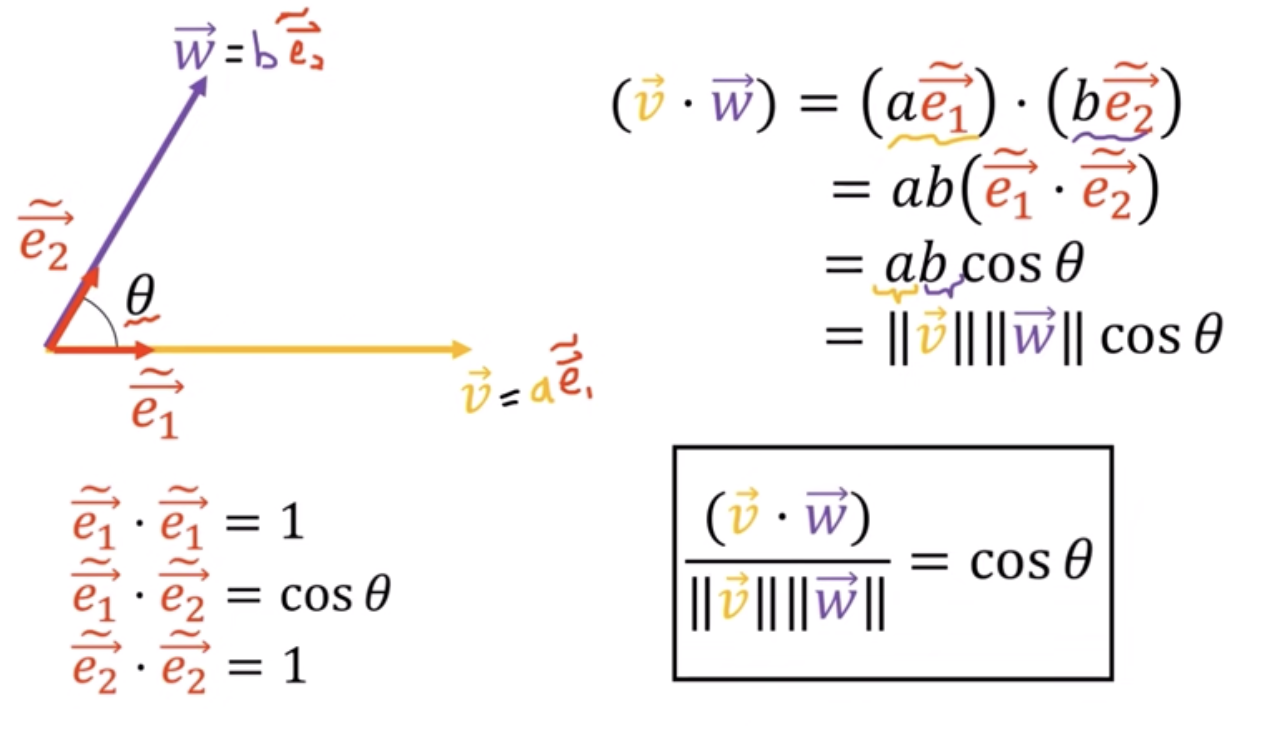
\includegraphics[width=0.6\textwidth]{Angle_between_vectors_dotproduct}
    \caption{Angle $\theta$ between two arbitrary vectors.}
    \label{fig:angle_between_arbitrary_vectors}
\end{figure} \\

To check how the metric tensor transforms, we use the formulation of the metric tensor in
the new system and transform it by replacing the tilde-components by expressing them in
the old system via the definitions of the forward transform given by
equation~(\ref{eq:vector_trafo_overview}):

\begin{equation}
    \begin{array}{rcl}
        \tilde{g}_{ij} & = & \hdbtv{i} \cdot \hdbtv{j} \\
                       & = & (F^{k~}_{~i}\hdbv{k}) \cdot (F^{l~}_{~j}\hdbv{l}) \\
                       & = & F^{k~}_{~i}  F^{l~}_{~j} (\hdbv{k} \cdot \hdbv{l}) \\
        \Rightarrow\tilde{g}_{ij} & = & F^{k~}_{~i}  F^{l~}_{~j} {g}_{kl} \\
        \noalign{\vskip10pt}
        g_{kl} & = & \hdbv{k} \cdot \hdbv{l} \\
        & = & (B^{i~}_{~k}\hdbtv{i}) \cdot (B^{j~}_{~l}\hdbtv{j}) \\
        & = & B^{i~}_{~k} B^{j~}_{~l} (\hdbtv{i} \cdot \hdbtv{j}) \\
        \Rightarrow g_{kl} & = & B^{i~}_{~k} B^{j~}_{~l}  \tilde{g}_{ij}
    \end{array}
\end{equation} \\

\textcolor{red}{Metric tensors are (0,2)-tensors}, because they transform with covariant
transformation behaviour using two transformations for change from one system to another.
This is also suggested by using lower indices for the metric tensor components. \\


\newpage